% Reflection principle: a path from (0,2) to (16,4) that touches the axis (blue) and its reflection before the first visit to 0 (orange dashed), which starts at (0,-2). Generated by a short script.
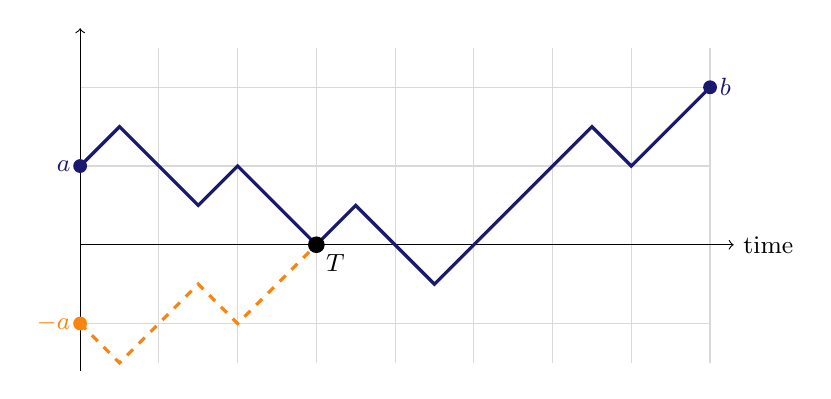
\begin{tikzpicture}[x=0.5cm,y=0.5cm]
\draw[black!15] (0,-3) grid (16,5);
\draw[->] (0,0)--(16.6,0) node[right,font=\small] {time};
\draw[->] (0,-3.2)--(0,5.5);
\draw[MidnightBlue,very thick] (0,2)--(1,3)--(2,2)--(3,1)--(4,2)--(5,1)--(6,0)--(7,1)--(8,0)--(9,-1)--(10,0)--(11,1)--(12,2)--(13,3)--(14,2)--(15,3)--(16,4);
\draw[BurntOrange,very thick,dashed] (0,-2)--(1,-3)--(2,-2)--(3,-1)--(4,-2)--(5,-1)--(6,0);
\fill[black] (6,0) circle (3pt) node[below right,font=\small] {$T$};
\fill[MidnightBlue] (0,2) circle (2.5pt) node[left,font=\small] {$a$};
\fill[BurntOrange] (0,-2) circle (2.5pt) node[left,font=\small] {$-a$};
\fill[MidnightBlue] (16,4) circle (2.5pt) node[right,font=\small] {$b$};
\end{tikzpicture}
